\chapter{Using \textsc{Larkita} as a Parser Generator  \label{chapter:ply}}
\epigraph{\blue{\large\calligfont Give a man a parser and he can read one programming language.} \\
          \blue{\large\calligfont Give a man a parser generator and he can read all programming languages.}}{--- Carlos Ben Yussuf}

\epigraph{\red{\large\calligfont Build a witch a fire and you keep her warm for one night.} \\
          \red{\large\calligfont Set a witch on fire and you keep her warm for the rest of her life.}}{--- Pope
        Hugo The Terrible}


\begin{figure}[h]
\centering
  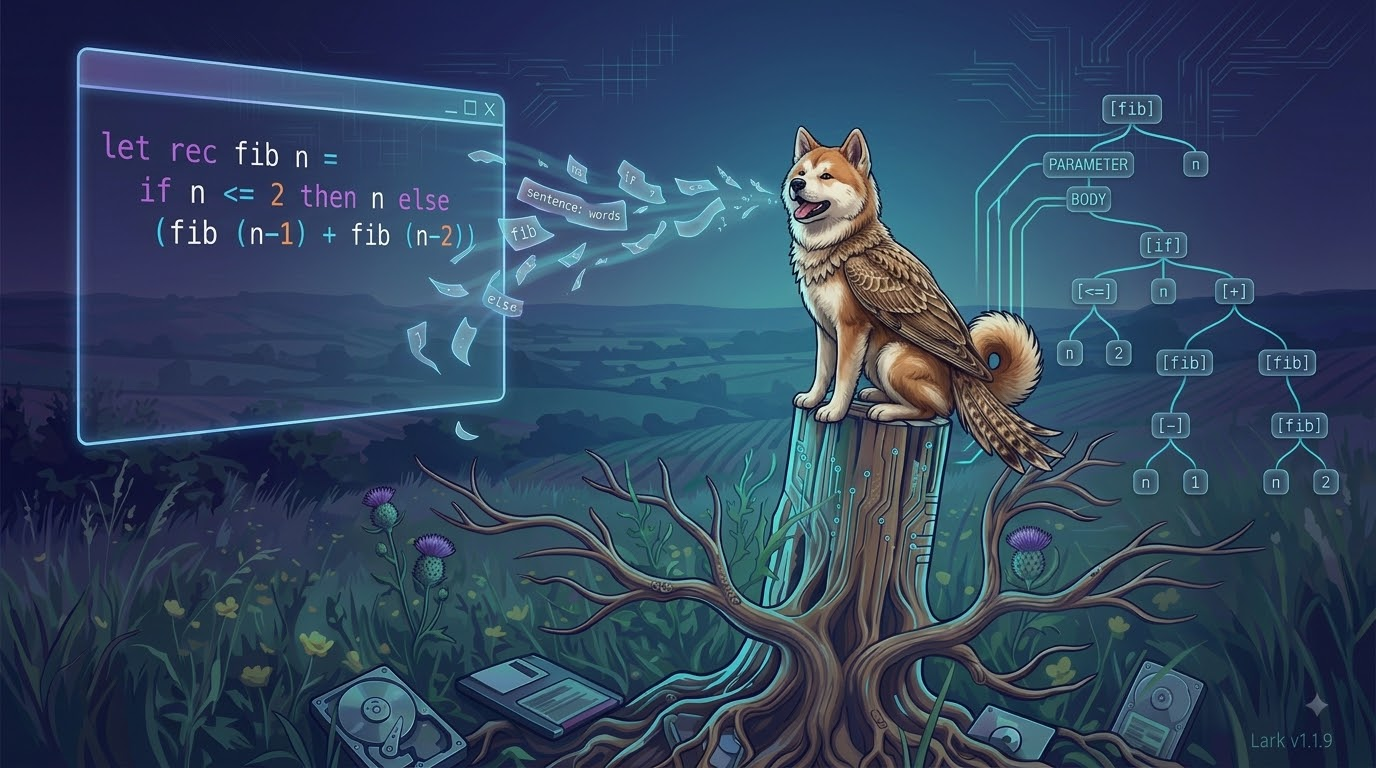
\includegraphics[width=17.0cm]{Abbildungen/larkita.png}
\caption{The Larkita parser generator in action.}
\label{fig:larkita.png}
\end{figure}
\pagebreak

Many modern programming languages, e.g.~\texttt{C}, \textsl{Java}, or \textsc{Go} can
be parsed using a so-called \blue{canonical LR(1)-Parser}\footnote{
  LR(1) is an acronym:  The input is read from \underline{L}eft to right, the parser constructs a
  \underline{R}ightmost derivation in reverse, and it uses \underline{1} token of lookahead.
  We will discuss the theory of canonical LR(1) parsing in Chapter \ref{chapter:bottom-up}.}.
Therefore, this chapter introduces the parser generator
\href{https://github.com/karlstroetmann/Larkita}{\simtextsc{Larkita}}\index{Larkita@\simtextsc{Larkita}}, which can
be used to generate a parser for any language that has an LR(1) grammar.\footnote{
  \simtextsc{Larkita} is a light-weight version of the parser generator
  \href{https://lark-parser.readthedocs.io/}{\simtextsc{Lark}}.  It is a pure \textsl{Python} library that can
  be installed via the command
  \\[0.1cm]
  \hspace*{1.3cm}
  \textcolor{amethyst}{\texttt{pip install larkita}}.}
In Chapter \ref{chapter:ply-lex} we have already seen how a scanner can be implemented with the help of the
module \texttt{re}.  \simtextsc{Larkita} goes one step further:  Both the \blue{lexical structure} and the
\blue{syntactical structure} of a language are described in a \emph{single} specification, and \simtextsc{Larkita}
generates the scanner \emph{and} the parser from this specification.  Hence, this chapter no longer has to
distinguish between the specification of a scanner and the specification of a parser.  Furthermore, the
grammar also determines the \blue{abstract syntax tree} that the parser returns:  This tree is represented as a
\blue{nested tuple}\index{nested tuple}, i.e.~it is an ordinary \textsl{Python} object.
We will discuss two examples that use \simtextsc{Larkita} as a parser generator.
\begin{enumerate}
\item First, we implement a symbolic calculator.  We implement it twice:  The first version uses a
      left-recursive grammar, while the second version uses a grammar with the operators of \simtextsc{Ebnf}.
\item In our second example, we develop a program for symbolic differentiation.
      This example shows how the abstract syntax tree that is returned by a parser can be transformed by a
      program.
\end{enumerate}
In Chapter \ref{chapter:interpreter} we will then use \simtextsc{Larkita} to create an interpreter for a language
that is a small fragment of the programming language \texttt{C}.

\remarkEng
Traditional parser generators for \textsl{Python}, for example
\href{https://www.dabeaz.com/ply/}{\simtextsc{Ply}}, encode every grammar rule as a \textsl{Python}
function whose \blue{document string} contains the grammar rule, and the
\blue{semantic action}\index{semantic action} associated with a 
rule is the body of this function.  Therefore, syntax and semantics are interleaved and hence they can't be
understood individually.  The parser generator \simtextsc{Larkita}
takes a different approach:  The grammar is written down as an ordinary string using a dialect of the
\blue{extended Backus-Naur form} \simtextsc{Ebnf}, and the grammar itself determines the abstract syntax tree
that is built.  The semantics is then implemented separately by functions that process this tree.  This
separation has two advantages:
\begin{itemize}
\item The grammar and the code for its interpretation are clearly separated, and 
\item the same grammar can be reused for different purposes.  \eox
\end{itemize}



\section{A Symbolic Calculator  \label{section:calculator}}
Figure \ref{fig:calculator.g} on page \pageref{fig:calculator.g} shows the grammar of a simple 
\blue{symbolic calculator}\index{calculator, symbolic}, i.e.~a calculator that supports the use of variables.  

\begin{figure}[!ht]

  \begin{center}    
  \framebox{
  \framebox{
  \begin{minipage}[t]{9cm}
  \begin{eqnarray*}
  \textsl{stmnt}   & \rightarrow & \;\simtextsc{Identifier} \quoted{:=} \textsl{expr} \quoted{;}\\
                   & \mid        & \;\textsl{expr} \quoted{;}                   \\[0.2cm]
  \textsl{expr}    & \rightarrow & \;\textsl{expr} \quoted{+} \textsl{product}  \\
                   & \mid        & \;\textsl{expr} \quoted{-} \textsl{product}  \\
                   & \mid        & \;\textsl{product}                           \\[0.2cm]
  \textsl{product} & \rightarrow & \;\textsl{product} \quoted{*} \textsl{factor}\\
                   & \mid        & \;\textsl{product} \quoted{/} \textsl{factor}\\
                   & \mid        & \;\textsl{factor}                            \\[0.2cm]
  \textsl{factor}  & \rightarrow &   \quoted{(} \textsl{expr} \quoted{)}        \\
                   & \mid        & \;\simtextsc{Number}                            \\
                   & \mid        & \;\simtextsc{Identifier}                        
  \end{eqnarray*}
  \vspace*{-0.5cm}
  \end{minipage}}}
  \end{center}
  \caption{A grammar for a symbolic calculator.}
  \label{fig:calculator.g}
\end{figure}

In order to generate a symbolic calculator that is based on this grammar, we have to transcribe the
grammar shown in Figure \ref{fig:calculator.g} into the \simtextsc{Ebnf} dialect that is understood by
\simtextsc{Larkita}.  Figure \ref{fig:01-Calculator.ipynb:grammar} on
page \pageref{fig:01-Calculator.ipynb:grammar} shows the result.  Note that there is no separate scanner
specification:  The terminals are declared inside the very same string that also declares the grammar
rules.

\begin{figure}[!ht]
\centering
\begin{minted}[ frame        = lines,
                framesep     = 0.3cm,
                bgcolor      = sepia,
                numbers      = left,
                numbersep    = 0.3cm,
                xleftmargin  = 0.3cm,
                xrightmargin = 0.3cm,
              ]{larkita_lexer.py:PythonLarkitaLexer}
    from larkita import Larkita

    calc_grammar = r"""
    stmnt: IDENTIFIER ":=" expr ";"
         | expr ";"

    expr: expr "+" product
        | expr "-" product
        | product

    product: product "*" factor
           | product "/" factor
           | factor

    factor: "(" expr ")"    %ignore "(", ")"
          | NUMBER
          | IDENTIFIER

    // Lexical definitions
    %import common.CNAME -> IDENTIFIER, common.NUMBER, common.WS

    // Ignore whitespace
    %ignore WS
    """

    parser = Larkita(calc_grammar, out_file='calc.out')
\end{minted}
\vspace*{-0.3cm}
\caption{The grammar of the symbolic calculator, written for \simtextsc{Larkita}.}
\label{fig:01-Calculator.ipynb:grammar}
\end{figure}

\noindent
Figure \ref{fig:01-Calculator.ipynb:grammar} is discussed line by line.
\begin{enumerate}
\item Line 1 imports the class \texttt{Larkita}, which is responsible for computing the parse table and for
      generating the parser.
\item Line 3 -- 24 define the string \texttt{calc\_grammar}.  Note that this is an ordinary
      \textsl{Python} string:  As far as \textsl{Python} is concerned, it has no structure at all.  Only
      when this string is handed to \simtextsc{Larkita} in line 26 is it interpreted as a grammar.

      \simtextsc{Larkita} distinguishes syntactical variables from tokens by their spelling:  The names of
      \blue{syntactical variables} have to be written in \textsl{lower case}, while the names of
      \blue{tokens} have to be written in \textsl{upper case}.  Therefore, \texttt{expr} is a syntactical
      variable, while \texttt{NUMBER} is a token.
\item Line 4 -- 5 define the syntactical variable \texttt{stmnt}.  This definition corresponds to the two
      grammar rules
      \\[0.2cm]
      \hspace*{1.3cm}
      $\textsl{stmnt} \rightarrow \simtextsc{Identifier} \quoted{:=} \textsl{expr} \quoted{;}$
      \quad and \quad
      $\textsl{stmnt} \rightarrow \textsl{expr} \quoted{;}$
      \\[0.2cm]
      of the grammar shown in Figure \ref{fig:calculator.g}.  Observe that the different alternatives of a
      rule are separated by the symbol ``\texttt{|}'', exactly as in the mathematical notation that we
      have used so far, and that literal strings like \squoted{:=} are simply written down as
      \textsl{Python} strings.

      As \texttt{stmnt} is the first syntactical variable of the grammar, it is the \blue{start symbol}.
\item Line 7 -- 13 define the variables \texttt{expr} and \texttt{product}.  These rules are literal
      transcriptions of the corresponding rules of Figure \ref{fig:calculator.g}.  In particular, they
      encode the \blue{precedence}\index{precedence!of arithmetic operators} of the arithmetic operators, and they are \blue{left recursive}.
      Left recursion is not a problem here, since LR parsing is a \blue{bottom-up} technique.
\item Line 15 -- 17 define the variable \texttt{factor}.  The annotation \texttt{\%ignore "(", ")"} at the end
      of line 15 is explained below, when we discuss the abstract syntax tree.
\item Line 20 imports predefined token definitions from the library \texttt{common} that is shipped
      with \simtextsc{Larkita}.  Several imports are separated by commas.  Instead of writing our own regular
      expressions we reuse the following definitions:
      \begin{enumerate}
      \item \texttt{CNAME} matches an identifier in the sense of the language \texttt{C}.  The construct
            ``\texttt{-> IDENTIFIER}'' renames this token to \texttt{IDENTIFIER}.
      \item \texttt{NUMBER} matches both integers and floating point numbers.
      \item \texttt{WS} matches \blue{white space}, i.e.~blanks, tabulators, and newlines.
      \end{enumerate}
\item Line 23 instructs the scanner to discard all white space.
\item Line 26 creates the parser.  It is at this point that the parse table is computed.
      By default, \simtextsc{Larkita} computes the parse table of a \blue{canonical LR(1) parser}.  If the given
      grammar is not an LR(1) grammar, then the parse table has conflicts.  We will discuss in Chapter
      \ref{chapter:bottom-up} what this means and how \simtextsc{Larkita} deals with conflicts.

      Furthermore, \simtextsc{Larkita} writes a description of all states of the parser into the file that is
      specified by the keyword argument \texttt{out\_file}, which is the file \texttt{calc.out} here.
\end{enumerate}
\FloatBarrier

\noindent
Once the parser has been created, a string \texttt{s} can be parsed by evaluating the expression
\\[0.2cm]
\hspace*{1.3cm}
\texttt{parser.parse(s)}.
\\[0.2cm]
This expression returns the \blue{abstract syntax tree} of \texttt{s}, which is represented as a
\blue{nested tuple}.  The shape of this tuple is determined by the grammar.  If a string has been parsed with
an alternative of a grammar rule, then the tuple that is built for this alternative is constructed as follows.
\begin{enumerate}
\item The string literals of the alternative form the \blue{head}\index{head (Larkita)@head (\simtextsc{Larkita})}
      of the tuple, i.e.~its first component.  If the alternative contains exactly one literal, the head is
      this literal.  If it contains several literals, the head is the tuple of these literals in the order in
      which they are written.
\item All other symbols of the alternative become the \blue{children} of the tuple, i.e.~its remaining
      components:  For a syntactical variable, the child is its abstract syntax tree, while a named token like
      \texttt{NUMBER} yields a pair consisting of the name of the token and the text that has been read.
      For example, the number 42 yields the pair
      \\[0.2cm]
      \hspace*{1.3cm}
      \texttt{('NUMBER', '42')}.
\item If an alternative has no head and consists of a single symbol, then no new tuple is built.  Instead,
      the abstract syntax tree of this symbol is returned.  Hence, alternatives like \texttt{expr: product} or
      \texttt{product: factor} leave no trace in the abstract syntax tree.
\item The annotation \texttt{\%ignore "(", ")"} at the end of an alternative removes the given literals from
      the head of this alternative.  Hence, the alternative \texttt{"(" expr ")"} in line 15 consists of a
      single symbol and returns the abstract syntax tree of \texttt{expr}.  This is exactly what we want,
      because the only purpose of the parentheses is to override the precedence of the operators.  Note
      that this annotation is unrelated to the directive \texttt{\%ignore WS} in line 23, which tells the
      scanner to discard white space.
\end{enumerate}
For example, the alternative \texttt{expr "+" product} yields the tuple
\\[0.2cm]
\hspace*{1.3cm}
\texttt{('+', $\textsl{ast}_1$, $\textsl{ast}_2$)},
\\[0.2cm]
where $\textsl{ast}_1$ and $\textsl{ast}_2$ are the abstract syntax trees of \texttt{expr} and \texttt{product},
while the alternative \texttt{IDENTIFIER ":=" expr ";"} yields
\\[0.2cm]
\hspace*{1.3cm}
\texttt{((':=', ';'), ('IDENTIFIER', $\textsl{name}$), $\textsl{ast}$)}.

\exampleEng
The string
\\[0.2cm]
\hspace*{1.3cm}
\texttt{"x := 2 * (y + 1);"}
\\[0.2cm]
is parsed into the nested tuple
\\[0.2cm]
\hspace*{0.3cm}
\texttt{((':=', ';'), ('IDENTIFIER', 'x'),}
\\
\hspace*{0.8cm}
\texttt{('*', ('NUMBER', '2'), ('+', ('IDENTIFIER', 'y'), ('NUMBER', '1'))))}.
\\[0.2cm]
Note the following details:
\begin{enumerate}
\item The parentheses of the input string have disappeared, since they are already reflected by the
      structure of the tuple.
\item The tokens are represented as pairs.  Hence, the identifier \texttt{x} on the left hand side of the
      assignment operator is represented by the tuple \texttt{('IDENTIFIER', 'x')}.
\item The numbers are still represented as strings.  They are converted into floating point numbers only
      when the abstract syntax tree is evaluated. \eox
\end{enumerate}

\noindent
Note that the abstract syntax tree returned by \texttt{parser.parse} does not know anything about the
\emph{meaning} of the program that has been parsed.  Providing this meaning is our job:  We have to evaluate
the nested tuple.  As the abstract syntax tree is a \blue{pure} \textsl{Python} object, we can inspect it, print
it, or store it without having to know anything about the internals of the parser.

\begin{figure}[!ht]
\centering
\begin{minted}[ frame        = lines,
                framesep     = 0.3cm,
                bgcolor      = sepia,
                numbers      = left,
                numbersep    = 0.3cm,
                xleftmargin  = 0.0cm,
                xrightmargin = 0.0cm,
                gobble       = 3,
              ]{python3}
   Names2Values = {}

   def evaluate_adt(adt):
       match adt:
           case ('NUMBER', value):
               return float(value)
           case ('IDENTIFIER', var_name):
               if var_name not in Names2Values:
                   print(f"Error: variable '{var_name}' is undefined.")
                   return 0.0
               return Names2Values[var_name]
           case ((':=', ';'), ('IDENTIFIER', var_name), expr):
               Names2Values[var_name] = evaluate_adt(expr)
           case (';', expr):
               print(evaluate_adt(expr))
           case (('+' | '-' | '*' | '/') as op, left, right):
               val_left  = evaluate_adt(left )
               val_right = evaluate_adt(right)
               match op:
                   case '+': return val_left + val_right
                   case '-': return val_left - val_right
                   case '*': return val_left * val_right
                   case '/': return val_left / val_right
           case _:
               raise ValueError(f"Unknown ADT structure: {adt}")
\end{minted}
\vspace*{-0.3cm}
\caption{Evaluating the abstract syntax tree.}
\label{fig:01-Calculator.ipynb:eval}
\end{figure}

\noindent
Figure \ref{fig:01-Calculator.ipynb:eval} on page \pageref{fig:01-Calculator.ipynb:eval} shows the
function \texttt{evaluate\_adt} that implements the semantics of our calculator.
\begin{enumerate}
\item Line 1 initializes the dictionary \texttt{Names2Values}.  For every identifier $x$ that is defined
      interactively, \texttt{Names2Values[$x$]} is the value associated with $x$.
\item Line 4 starts a \texttt{match} statement.  \blue{Structural pattern matching}\index{pattern matching} is the natural way to
      work with an abstract syntax tree that is represented as a nested tuple:  Every case of the
      \texttt{match} statement corresponds to one of the shapes that occur in our abstract syntax tree.
\item Line 5 -- 6 evaluate a number.  This is the place where the string produced by the scanner is
      converted into a floating point number.
\item Line 7 -- 11 evaluate a variable.  If the variable has not been defined previously, an error message
      is printed and the value $0.0$ is returned.
\item Line 12 -- 13 implement an assignment:  The expression on the right hand side is evaluated and the
      resulting value is stored in the dictionary \texttt{Names2Values}.  Note that the pattern in line 12
      extracts the name of the variable from the token \texttt{('IDENTIFIER', var\_name)} and that an
      assignment does not return a value.
\item Line 14 -- 15 implement an expression statement:  The expression is evaluated and the resulting value
      is printed.
\item Line 16 -- 23 evaluate the arithmetic operators.  The pattern in line 16 uses an \blue{or pattern}\index{pattern matching!or pattern} in
      order to capture all four binary operators at once.  The keyword \texttt{as} binds the operator that
      has actually been found to the variable \texttt{op}.  Then, both operands are evaluated recursively
      and the inner \texttt{match} statement in line 19 -- 23 selects the operation that has to be
      performed.
\item Line 24 -- 25 catch the case that the abstract syntax tree has a shape that is not supported.  If
      this happens, we have made a mistake, either in the grammar or in the function
      \texttt{evaluate\_adt}.
\end{enumerate}
\FloatBarrier

\begin{figure}[!ht]
\centering
\begin{minted}[ frame        = lines,
                framesep     = 0.3cm,
                bgcolor      = sepia,
                gobble       = 4,
                numbers      = left,
                numbersep    = 0.3cm,
                xleftmargin  = 0.0cm,
                xrightmargin = 0.0cm,
              ]{python3}
    def main():
        while True:
            try:
                s = input('calc> ')
                if s == '':
                    break
                # 1. Parse the string into a nested tuple
                adt = parser.parse(s)
                # 2. Evaluate the nested tuple
                evaluate_adt(adt)
            except (EOFError, NotImplementedError):  # no input possible
                break
            except Exception as e:
                print(f"Error: {e}")
\end{minted}
\vspace*{-0.3cm}
\caption{A read-eval-print loop for the symbolic calculator.}
\label{fig:01-Calculator.ipynb:main}
\end{figure}

\noindent
Finally, Figure \ref{fig:01-Calculator.ipynb:main} on page \pageref{fig:01-Calculator.ipynb:main} shows
the function \texttt{main}, which is a \blue{read-eval-print loop}\index{read-eval-print loop}:  It reads a string \texttt{s} from the
command line and then performs the two steps that we have discussed:  Line 8 parses the string into a nested
tuple and line 10 evaluates this tuple.  The loop is terminated as soon as the user enters an empty line.  It is
also terminated if no input can be read at all:  Then the function \texttt{input} raises an \texttt{EOFError}
or, inside a Jupyter notebook that is executed automatically, a \texttt{NotImplementedError}.  Line 11 -- 12
catch these exceptions.

Observe how \simtextsc{Larkita} reports errors:  Instead of calling an error function that has been provided
by the user, \simtextsc{Larkita} raises an \blue{exception}.  Both lexical errors and syntax errors are
signalled by subclasses of the class \texttt{larkita.UnexpectedInput}.  As these exceptions carry
the position where the error has occurred, the messages produced by \simtextsc{Larkita} are usually much more
informative than the messages that we could produce ourselves with a modest amount of effort.  The
\texttt{try}-\texttt{except} statement in line 3 and line 13 -- 14 catches these exceptions so that a
single erroneous input does not terminate the calculator.

The Jupyter notebook \texttt{01-Calculator}, which is available at
\\[0.2cm]
\hspace*{1.3cm}
\href{https://github.com/karlstroetmann/Formal-Languages/blob/master/Python/Chapter-07/01-Calculator.ipynb}{Python/Chapter-07/01-Calculator.ipynb}
\\[0.2cm]
implements the symbolic calculator discussed in this section.

\remarkEng
The notebook \texttt{01-Calculator} also prints the file \texttt{calc.out}, which describes all states of the
LR(1) parser that has been computed by \simtextsc{Larkita}.  At this point, these states will not make much
sense.  However, it is worthwhile to return to this part of the notebook once we have discussed the theory of
LR(1) parsing in Chapter \ref{chapter:bottom-up}.  \eox

\exerciseEng
Extend the grammar shown in Figure \ref{fig:01-Calculator.ipynb:grammar} so that the calculator supports
the \blue{exponentiation operator} \squoted{**} and the \blue{unary minus}\index{unary minus}.  The exponentiation operator
binds stronger than multiplication and it is \blue{right associative}\index{right associative}, i.e.~the expression
\texttt{2 ** 3 ** 2} has the value $2^{(3^2)} = 512$.  Furthermore, extend the function
\texttt{evaluate\_adt} accordingly.
\\[0.2cm]
\hint
Introduce a new syntactical variable \texttt{power} between \texttt{product} and \texttt{factor} and make
this variable right recursive.  The section on symbolic differentiation shows how an \blue{alias} can be used
to distinguish the unary minus from the binary minus.

\section{A Calculator with an \texorpdfstring{\simtextsc{Ebnf}}{EBNF} Grammar  \label{section:calculator-ebnf}}
The grammar shown in Figure \ref{fig:01-Calculator.ipynb:grammar} is a literal transcription of the
left-recursive grammar of Figure \ref{fig:calculator.g}.  In Section \ref{section:recursive-descent-ebnf} we
have seen that an expression can also be described as a sequence of products that are separated by the
operators \squoted{+} and \squoted{-}, and that a product can be described as a sequence of factors that are
separated by the operators \squoted{*} and \squoted{/}.  This leads to the \simtextsc{Ebnf} grammar shown in
Figure \ref{fig:arith-expr-ebnf} on page \pageref{fig:arith-expr-ebnf}.  As \simtextsc{Larkita} supports
the operators of \simtextsc{Ebnf}, we can use this grammar directly.  Figure
\ref{fig:01-Calculator-EBNF.ipynb:grammar} shows the grammar of the symbolic calculator written in this
style.  Only the rules for \texttt{expr} and \texttt{product} have changed.  The lexical definitions are the
same as in Figure \ref{fig:01-Calculator.ipynb:grammar} and are therefore not shown again.

\begin{figure}[!ht]
\centering
\begin{minted}[ frame        = lines,
                framesep     = 0.3cm,
                bgcolor      = sepia,
                gobble       = 4,
                numbers      = left,
                numbersep    = 0.3cm,
                xleftmargin  = 0.8cm,
                xrightmargin = 0.8cm,
              ]{larkita_lexer.py:PythonLarkitaLexer}
    calc_grammar = r"""
    stmnt: IDENTIFIER ":=" expr ";"
         | expr ";"

    expr: product (("+" | "-") product)*

    product: factor (("*" | "/") factor)*

    factor: "(" expr ")"    %ignore "(", ")"
          | NUMBER
          | IDENTIFIER
\end{minted}
\vspace*{-0.3cm}
\caption{The grammar of the symbolic calculator, written with \simtextsc{Ebnf} operators.}
\label{fig:01-Calculator-EBNF.ipynb:grammar}
\end{figure}

\noindent
The rules in line 5 and line 7 use two operators of \simtextsc{Ebnf}.
\begin{enumerate}
\item The postfix operator ``\texttt{*}'' denotes a \blue{repetition}\index{repetition (\simtextsc{Ebnf})}:
      The part in parentheses can occur any number of times, including zero times.  Similarly, the postfix
      operator ``\texttt{+}'' denotes one or more repetitions, while a part that is enclosed in square brackets
      is optional.  These operators are used in Chapter \ref{chapter:interpreter}.
\item The part \verb!("+" | "-")! is an \blue{inner alternative}\index{inner alternative}, i.e.~an
      alternative that occurs inside an alternative of a grammar rule.  An inner alternative has to be enclosed
      in parentheses.
\end{enumerate}
Hence, line 5 states that an expression is a product that is followed by any number of pairs, where every
pair consists of one of the operators \squoted{+} or \squoted{-} and another product.  This single rule
replaces the three rules for \texttt{expr} in Figure \ref{fig:01-Calculator.ipynb:grammar}.

When an alternative contains repetitions or inner alternatives, the rules for building the abstract syntax
tree that have been given in Section \ref{section:calculator} are complemented as follows.
\begin{enumerate}
\item The children that are produced by the repeated parts are \blue{spliced}\index{splicing (\simtextsc{Larkita})}
      into the tuple of the alternative.  Hence, the alternative in line 5 builds a single \emph{flat} tuple
      that contains all products of the expression, no matter how many products there are.
\item The head of a tuple is determined by the grammar, not by the input.  Inside a repetition, the head
      cannot record which operator has been read, since a single tuple contains all the operators.
      Therefore, the literals of an inner alternative that occurs inside a repetition do not belong to the
      head.  Instead, the literal that has actually been read becomes a child of the tuple.  As it is a literal
      and not a named token, it is represented by a plain string like \texttt{'-'} rather than by a pair.
\item The alternative in line 5 has no literal that belongs to the head.  As it contains a repetition, it does
      not return the abstract syntax tree of one of its symbols either.  In this case, the name of the rule is
      used as the head.  Therefore, the alternative in line 5 builds tuples of the form
      \\[0.2cm]
      \hspace*{1.3cm}
      \texttt{('expr', $p_1$, $o_1$, $p_2$, $\cdots$, $o_{n-1}$, $p_n$)},
      \\[0.2cm]
      where $p_1$, $\cdots$, $p_n$ are the abstract syntax trees of the products and $o_1$, $\cdots$,
      $o_{n-1}$ are the operators.  Since the shape of the tuple is determined by the grammar, an expression
      that consists of a single product is represented as \texttt{('expr', $p_1$)}.
\item An inner alternative that does \emph{not} occur inside a repetition or inside an optional part is
      nothing but an abbreviation.  For example, the alternative
      \\[0.2cm]
      \hspace*{1.3cm}
      \verb!expr: expr ("+" | "-") product!
      \\[0.2cm]
      stands for the two alternatives \texttt{expr "+" product} and \texttt{expr "-" product}.  Hence, the
      operator that has been read is the head, and this alternative yields the same tuples as the rules for
      \texttt{expr} in Figure \ref{fig:01-Calculator.ipynb:grammar}.  Chapter \ref{chapter:interpreter} uses
      inner alternatives in this way.
\end{enumerate}

\exampleEng
The string
\\[0.2cm]
\hspace*{1.3cm}
\texttt{"1 - 2 * 3 - 4;"}
\\[0.2cm]
is parsed into the nested tuple
\\[0.2cm]
\hspace*{0.3cm}
\texttt{(';', ('expr',}
\\
\hspace*{0.8cm}
\texttt{('product', ('NUMBER', '1')),}
\\
\hspace*{0.8cm}
\texttt{'-', ('product', ('NUMBER', '2'), '*', ('NUMBER', '3')),}
\\
\hspace*{0.8cm}
\texttt{'-', ('product', ('NUMBER', '4'))))}.
\\[0.2cm]
The three products and the two operators are the children of a single tuple with the head \squoted{expr}. \eox

\noindent
The flat tuples do not specify how the operands are grouped.  As discussed in Section
\ref{section:recursive-descent-ebnf}, the \simtextsc{Ebnf} rule for \texttt{expr} merely states that an expression
is a sequence of products.  It no longer expresses that the operator \squoted{-} is left associative.
Therefore, we have to group the operands ourselves.  The function \texttt{to\_binary} that is shown in
Figure \ref{fig:01-Calculator-EBNF.ipynb:to_binary} on page \pageref{fig:01-Calculator-EBNF.ipynb:to_binary}
converts the flat tuples into the binary tuples of Section \ref{section:calculator}.

\begin{figure}[!ht]
\centering
\begin{minted}[ frame        = lines,
                framesep     = 0.3cm,
                bgcolor      = sepia,
                gobble       = 4,
                numbers      = left,
                numbersep    = 0.3cm,
                xleftmargin  = 0.0cm,
                xrightmargin = 0.0cm,
              ]{python3}
    def to_binary(ast):
        match ast:
            case ('NUMBER' | 'IDENTIFIER', _):
                return ast
            case ('expr' | 'product', first, *rest):
                # Combine the operands of a flat tuple from left to right
                result = to_binary(first)
                for op, operand in zip(rest[0::2], rest[1::2]):
                    result = (op, result, to_binary(operand))
                return result
            case (head, *children):
                return (head, *[to_binary(child) for child in children])
\end{minted}
\vspace*{-0.3cm}
\caption{Converting the flat tuples into binary tuples.}
\label{fig:01-Calculator-EBNF.ipynb:to_binary}
\end{figure}

\begin{enumerate}
\item Line 3 -- 4 return the tuples that represent tokens unchanged.
\item Line 5 -- 10 convert a flat tuple.  The pattern in line 5 binds the first operand to the variable
      \texttt{first} and the list of all remaining children to the variable \texttt{rest}.  This list has the
      form $[o_1, p_2, o_2, p_3, \cdots, o_{n-1}, p_n]$.  Hence, the slice \texttt{rest[0::2]} contains the
      operators, while the slice \texttt{rest[1::2]} contains the remaining operands.  Line 9 builds a new
      binary tuple whose left operand is the tree that has been built so far.  This is exactly what the
      \texttt{while} loop of the function \texttt{parseExpr} shown in Figure \ref{fig:2-EBNF-Parser-AST.ipynb}
      does:  The operands are grouped from left to right.  If the flat tuple contains a single operand, then
      the loop is not executed and the abstract syntax tree of this operand is returned.  Therefore, a tuple
      like \texttt{('expr', $p_1$)} leaves no trace in the result.
\item Line 11 -- 12 convert all other tuples, i.e.~the tuples that represent statements:  Their head is kept and
      their children are converted recursively.
\end{enumerate}
For example, the nested tuple of the previous example is converted into
\\[0.2cm]
\hspace*{0.3cm}
\texttt{(';', ('-', ('-', ('NUMBER', '1'),}
\\
\hspace*{4.68cm}
\texttt{('*', ('NUMBER', '2'), ('NUMBER', '3'))),}
\\
\hspace*{3.21cm}
\texttt{('NUMBER', '4')))},
\\[0.2cm]
which represents the expression \texttt{(1 - 2 * 3) - 4}.  This is the same tuple that is returned by the
parser of Section \ref{section:calculator}.  Therefore, the function \texttt{evaluate\_adt} shown in Figure
\ref{fig:01-Calculator.ipynb:eval} can be used without any change.  The read-eval-print loop differs from the
one shown in Figure \ref{fig:01-Calculator.ipynb:main} only in that it applies the function
\texttt{to\_binary} to the nested tuple before it evaluates the tuple.

The Jupyter notebook \texttt{01-Calculator-EBNF}, which is available at
\\[0.2cm]
\hspace*{1.3cm}
\href{https://github.com/karlstroetmann/Formal-Languages/blob/master/Python/Chapter-07/01-Calculator-EBNF.ipynb}{Python/Chapter-07/01-Calculator-EBNF.ipynb}
\\[0.2cm]
implements the calculator discussed in this section.

\remarkEng
The parse table of an LR(1) parser is computed from grammar rules that do not use the operators of
\simtextsc{Ebnf}.  Therefore, \simtextsc{Larkita} translates the repetition in line 5 into a new syntactical
variable \texttt{\_\_expr\_star\_0} that is defined by left-recursive rules.  These rules show up in the file
\texttt{calc-ebnf.out}, which is printed by the notebook.  The reductions with these rules do not build tuples
of their own.  Instead, they collect the children of the repeated parts in a list, which is then spliced into
the tuple of the alternative in line 5.  \eox

\section{Symbolic Differentiation  \label{section:differentiator}}
Our second example shows how a parser can be used to construct an \blue{abstract syntax tree} that is
afterwards transformed by a program.  Concretely, we implement \blue{symbolic differentiation}\index{symbolic differentiation}:  Given a
string \texttt{s} that represents an arithmetic expression containing the variable \texttt{x}, we want to
compute a string that represents the derivative
\\[0.2cm]
\hspace*{1.3cm}
$\ds\frac{\mathrm{d}\;}{\mathrm{d}x} \texttt{s}$.
\\[0.2cm]
For example, given the input string \texttt{"x*exp(x)"} the program should produce the output string
\\[0.2cm]
\hspace*{1.3cm}
\texttt{"exp(x) + x*exp(x)"}
\\[0.2cm]
since we have
\\[0.2cm]
\hspace*{1.3cm}
$\ds\frac{\mathrm{d}\;}{\mathrm{d}x} \bigl( x \cdot \mathrm{e}^x \bigr) = \mathrm{e}^x + x \cdot \mathrm{e}^x$.
\\[0.2cm]
In contrast to the calculator of the previous section, the abstract syntax tree is no longer evaluated
immediately.  Instead, it is the \emph{data} that our program works on:  It is transformed into a second
abstract syntax tree that represents the derivative, this tree is then simplified, and only at the very
end is it converted back into a string.  This is the reason why building an explicit abstract syntax tree
pays off.

Figure \ref{fig:differentiator.g} on page \pageref{fig:differentiator.g} shows the grammar of the
arithmetic expressions that our program supports.  Besides the four basic arithmetic operators, this
grammar supports the \blue{exponentiation operator} \squoted{**}, the \blue{unary minus}, and the two
functions $\exp$ and $\ln$.  For the sake of simplicity, \texttt{x} is the only variable.

\begin{figure}[!ht]

  \begin{center}    
  \framebox{
  \framebox{
  \begin{minipage}[t]{10cm}
  \begin{eqnarray*}
  \textsl{expr}    & \rightarrow & \;\textsl{expr} \quoted{+} \textsl{product}      \\
                   & \mid        & \;\textsl{expr} \quoted{-} \textsl{product}      \\
                   & \mid        & \;\textsl{product}                               \\[0.2cm]
  \textsl{product} & \rightarrow & \;\textsl{product} \quoted{*} \textsl{unary}     \\
                   & \mid        & \;\textsl{product} \quoted{/} \textsl{unary}     \\
                   & \mid        & \;\textsl{unary}                                 \\[0.2cm]
  \textsl{unary}   & \rightarrow &   \quoted{-} \textsl{unary}                      \\
                   & \mid        & \;\textsl{factor}                                \\[0.2cm]
  \textsl{factor}  & \rightarrow & \;\textsl{base} \quoted{**} \textsl{unary}       \\
                   & \mid        & \;\textsl{base}                                  \\[0.2cm]
  \textsl{base}    & \rightarrow &   \quoted{exp} \quoted{(} \textsl{expr} \quoted{)} \\
                   & \mid        &   \quoted{ln} \quoted{(} \textsl{expr} \quoted{)}  \\
                   & \mid        &   \quoted{(} \textsl{expr} \quoted{)}            \\
                   & \mid        & \;\simtextsc{Number}                             \\
                   & \mid        &   \quoted{x}                                     
  \end{eqnarray*}
  \vspace*{-0.5cm}
  \end{minipage}}}
  \end{center}
  \caption{A grammar for differentiable arithmetic expressions.}
  \label{fig:differentiator.g}
\end{figure}

\noindent
Figure \ref{fig:02-Differentiator.ipynb:grammar} on page \pageref{fig:02-Differentiator.ipynb:grammar}
shows the transcription of this grammar into the \simtextsc{Ebnf} dialect of \simtextsc{Larkita}.

\begin{figure}[!ht]
\centering
\begin{minted}[ frame        = lines,
                framesep     = 0.3cm,
                bgcolor      = sepia,
                numbers      = left,
                numbersep    = 0.3cm,
                xleftmargin  = 0.8cm,
                xrightmargin = 0.8cm,
              ]{larkita_lexer.py:PythonLarkitaLexer}
    from larkita import Larkita

    calc_grammar = r"""
    expr: expr "+" product
        | expr "-" product
        | product

    product: product "*" unary
           | product "/" unary
           | unary

    unary: "-" unary            -> neg
         | factor

    factor: base "**" unary
          | base

    base: "exp" "(" expr ")"    -> exp
        | "ln" "(" expr ")"     -> ln
        | "(" expr ")"          %ignore "(", ")"
        | NUMBER
        | "x"

    %import common.NUMBER, common.WS
    %ignore WS
    """

    parser = Larkita(calc_grammar, out_file='diff.out')
\end{minted}
\vspace*{-0.3cm}
\caption{The grammar of the differentiator, written for \simtextsc{Larkita}.}
\label{fig:02-Differentiator.ipynb:grammar}
\end{figure}

\noindent
As the general structure of this grammar is the same as the structure of the grammar that we have
discussed in the previous section, we only comment on those parts that are new.
\begin{enumerate}
\item Line 4 -- 10 define the variables \texttt{expr} and \texttt{product} in the usual way.  As
      \texttt{expr} is the first variable of the grammar, it is the start symbol.  In contrast to the
      calculator, this language has no statements:  The input is a single expression and there is no
      terminating semicolon.  Note that the second operand of the operators \squoted{*} and \squoted{/} is
      now the variable \texttt{unary} instead of the variable \texttt{factor}.
\item Line 12 -- 13 define the variable \texttt{unary}, which implements the \blue{unary minus}.  This rule
      is \blue{right recursive}\index{right recursive}, since a unary operator can be applied repeatedly:  The string
      \texttt{"-\,-x"} is a legal expression.

      The construct ``\texttt{-> neg}'' at the end of line 12 is an
      \blue{alias}\index{alias (Larkita)@alias (\simtextsc{Larkita})}.  An alias replaces the head of the tuple that is
      built for the alternative.  Without this alias, the head would be the literal \squoted{-} and a negation
      could only be distinguished from a subtraction by the number of components of its tuple.  With the alias,
      a negation is represented by a tuple of the form \texttt{('neg', $\textsl{ast}$)}.
\item Line 15 -- 16 define the variable \texttt{factor}, which implements exponentiation.  The interplay
      between \texttt{unary} and \texttt{factor} deserves a closer look, because it encodes two
      conventions that every mathematician takes for granted:
      \begin{enumerate}
      \item The left operand of the operator \squoted{**} is a \texttt{base}, not a \texttt{unary} operator.
            Therefore, the string
            \\[0.2cm]
            \hspace*{1.3cm}
            \texttt{"-x ** 2"}
            \\[0.2cm]
            is parsed as $-\bigl(x^2\bigr)$ and not as
            $(-x)^2$, i.e.~exponentiation binds stronger than the unary minus.
      \item The right operand of the operator \squoted{**} is a \texttt{unary}, not a \texttt{base}.
            Therefore, the string
            \\[0.2cm]
            \hspace*{1.3cm}
            \texttt{"x ** -x"}
            \\[0.2cm]
            is a legal expression and, furthermore, the operator
            \squoted{**} is \blue{right associative}:  The string
            \\[0.2cm]
            \hspace*{1.3cm}
            \texttt{"x ** x ** x"}
            \\[0.2cm] is parsed as the expression $x^{\left(x^x\right)}$.
      \end{enumerate}
\item Line 18 -- 22 define the variable \texttt{base}.  The strings \texttt{"exp"} and \texttt{"ln"} in
      line 18 and line 19 are ordinary literals, i.e.~they are recognized in exactly the same way as the
      operator symbols.  Without the aliases \texttt{exp} and \texttt{ln}, the heads of these alternatives
      would be the tuples
      \\[0.2cm]
      \hspace*{1.3cm}
      \texttt{('exp', '(', ')')} \quad and \quad \texttt{('ln', '(', ')')}.
      \\[0.2cm]
      With the aliases, the abstract syntax tree of the string \texttt{"exp(x)"} is the pair
      \texttt{('exp', $\textsl{ast}$)}.
\item Line 22 shows that the only variable of our expressions is \texttt{x}.  Since \texttt{x} is written
      as a literal string, we do not need a token for identifiers at all.  As this alternative consists of a
      single literal, its abstract syntax tree is the tuple \texttt{('x',)}, which has the head \squoted{x} and
      no children.
\end{enumerate}
\FloatBarrier

\noindent
For example, the string \texttt{"ln(x ** x) + exp(x * -x)"} is parsed into the nested tuple
\\[0.2cm]
\hspace*{0.3cm}
\texttt{('+', ('ln', ('**', ('x',), ('x',))),}
\\
\hspace*{0.8cm}
\texttt{('exp', ('*', ('x',), ('neg', ('x',)))))}.
\\[0.2cm]
The heads of these tuples are already the operator symbols that we want to use.  Only the \emph{leaves} of this
tree differ from the representation that our program for symbolic differentiation is going to use:  We want to
represent a number by the number itself and the variable \texttt{x} by the string \squoted{x}.
Figure \ref{fig:02-Differentiator.ipynb:ast} on page \pageref{fig:02-Differentiator.ipynb:ast} shows the
function \texttt{convert\_leaves} that converts the leaves, together with the function \texttt{parse} that
combines parsing and conversion.

\begin{figure}[!ht]
\centering
\begin{minted}[ frame        = lines,
                framesep     = 0.3cm,
                bgcolor      = sepia,
                numbers      = left,
                numbersep    = 0.3cm,
                xleftmargin  = 0.8cm,
                xrightmargin = 0.8cm,
                ]{python3}
    def convert_leaves(ast):
        match ast:
            case ('NUMBER', digits):
                return int(digits)
            case ('x',):
                return 'x'
            case (op, *args):
                return (op, *map(convert_leaves, args))

    def parse(s):
        return convert_leaves(parser.parse(s))
\end{minted}
\vspace*{-0.3cm}
\caption{Converting the leaves of the abstract syntax tree.}
\label{fig:02-Differentiator.ipynb:ast}
\end{figure}

\noindent
The function \texttt{convert\_leaves} is discussed next.
\begin{enumerate}
\item Line 3 -- 4 convert a number.  In contrast to the calculator of the previous section, the conversion
      of a string into a number happens already at this point, because the abstract syntax tree is not
      evaluated later but rather transformed symbolically.

      We will tacitly assume that all numbers are integers.
\item Line 5 -- 6 convert the variable \texttt{x}.
\item Line 7 is the most interesting line of this function.  The pattern \texttt{(op, *args)} matches every
      tuple that has at least one component.  The \blue{capture pattern}\index{pattern matching!capture pattern} \texttt{op}
      binds the head of the tuple to the variable \texttt{op}, while the \blue{star pattern}
      \texttt{*args} binds the list of the remaining components to the variable \texttt{args}.  Hence, this
      case is the default case that deals with all tuples that represent an operator or a function.
\item Line 8 converts all children recursively and prepends the head.  The expression
      \\[0.2cm]
      \hspace*{1.3cm}
      \texttt{map(convert\_leaves, args)}
      \\[0.2cm]
      applies the function \texttt{convert\_leaves} to every child, while the operator ``\texttt{*}'' unpacks
      the resulting iterator into the tuple that is created.  Note that this works for unary and for binary
      operators alike.
\item Line 10 -- 11 define the function \texttt{parse}, which combines both steps:  It parses the string
      \texttt{s} and immediately converts the leaves of the resulting abstract syntax tree.
\end{enumerate}

\exampleEng
The string \texttt{"ln(x ** x) + exp(x * -x)"} is converted into the nested tuple
\\[0.2cm]
\hspace*{0.3cm}
\texttt{('+', ('ln', ('**', 'x', 'x')), ('exp', ('*', 'x', ('neg', 'x'))))}.
\hspace*{\fill} $\diamond$

\remarkEng
As the heads of the tuples are determined by the grammar, it is usually sufficient to extend the grammar in
order to support an additional operator or an additional function:  If the alias of the new alternative is
already the symbol that we want to use in the abstract syntax tree, then the function
\texttt{convert\_leaves} does not have to be changed at all.  \eox
\vspace*{0.1cm}

\noindent
Now that we can turn a string into an abstract syntax tree, we are ready to implement the function
\texttt{diff}.  This function takes an abstract syntax tree $e$ and computes an abstract syntax tree that
represents the derivative of $e$ with respect to the variable \texttt{x}.  Figure
\ref{fig:02-Differentiator.ipynb:diff} on page \pageref{fig:02-Differentiator.ipynb:diff} shows the
implementation.  Every case of the \texttt{match} statement corresponds to one of the differentiation
rules that are taught in any calculus course.

\begin{figure}[!ht]
\centering
\begin{minted}[ frame        = lines, 
                framesep     = 0.3cm, 
                bgcolor      = sepia,
                numbers      = left,
                numbersep    = 0.4cm,
                xleftmargin  = 0.0cm,
                xrightmargin = 0.0cm,
              ]{python3}
def diff(e):
    "differentiate the expression e with respect to the variable x"
    match e:
        case ('+', f, g):
            fs, gs = diff(f), diff(g)
            return ('+', fs, gs)
        case ('-', f, g):
            fs, gs = diff(f), diff(g)
            return ('-', fs, gs)
        case ('*', f, g):
            fs, gs = diff(f), diff(g)
            return ('+', ('*', fs, g), ('*', f, gs))
        case ('/', f, g):
            fs, gs = diff(f), diff(g)
            return ('/', ('-', ('*',fs,g), ('*',f,gs)), ('*',g,g))
        case ('**', f, g):
            return diff(('exp', ('*', g, ('ln', f))))
        case ('neg', f):
            return ('neg', diff(f))
        case ('ln', f):
            fs = diff(f)
            return ('/', fs, f)
        case ('exp', f):
            fs = diff(f)
            return ('*', fs, e)
        case 'x':
            return 1
    return 0
\end{minted}
\vspace*{-0.3cm}
\caption{Symbolic differentiation.}
\label{fig:02-Differentiator.ipynb:diff}
\end{figure}

\noindent
The function \texttt{diff} is discussed next.
\begin{enumerate}
\item Line 4 -- 6 implement the \blue{sum rule}\index{differentiation!sum rule}
      $\ds\frac{\mathrm{d}\;}{\mathrm{d}x}\bigl(f(x) + g(x)\bigr) 
       = \frac{\mathrm{d}\;}{\mathrm{d}x} f(x) + \frac{\mathrm{d}\;}{\mathrm{d}x} g(x)$,
      \\[0.1cm]
      while line 7 -- 9 implement the corresponding rule for the difference of two expressions.
\item Line 10 -- 12 implement the \blue{product rule}\index{differentiation!product rule}
      \\[0.2cm]
      \hspace*{1.3cm}
      $\ds\frac{\mathrm{d}\;}{\mathrm{d}x}\bigl(f(x) \cdot g(x)\bigr)
       = \Bigl(\frac{\mathrm{d}\;}{\mathrm{d}x} f(x)\Bigr) \cdot g(x)
       + f(x) \cdot \Bigl(\frac{\mathrm{d}\;}{\mathrm{d}x} g(x)\Bigr)$.
\item Line 13 -- 15 implement the \blue{quotient rule}\index{differentiation!quotient rule}
      \\[0.2cm]
      \hspace*{1.3cm}
      $\ds\frac{\mathrm{d}\;}{\mathrm{d}x}\left(\frac{f(x)}{g(x)}\right)
       = \frac{\Bigl(\frac{\mathrm{d}}{\mathrm{d}x} f(x)\Bigr) \cdot g(x)
              - f(x) \cdot \Bigl(\frac{\mathrm{d}}{\mathrm{d}x} g(x)\Bigr)}{g(x) \cdot g(x)}$.
\item Line 16 -- 17 deal with exponentiation.  Instead of implementing a separate rule for the expression
      $f(x)^{g(x)}$, we use the identity
      \\[0.2cm]
      \hspace*{1.3cm}
      $f(x)^{g(x)} = \exp\bigl(g(x) \cdot \ln(f(x))\bigr)$
      \\[0.2cm]
      and differentiate the resulting expression instead.  This is an instance of a general and very
      useful strategy:  Rather than adding a new rule, we \blue{rewrite} the expression so that it can be
      handled by the rules that we already have.  Note that this identity is only valid if $f(x)$ is
      positive.  Our implementation ignores this side condition.
\item Line 18 -- 19 implement the rule
      $\ds\frac{\mathrm{d}\;}{\mathrm{d}x}\bigl(-f(x)\bigr) 
       = -\frac{\mathrm{d}\;}{\mathrm{d}x} f(x)$.
\item Line 20 -- 22 and line 23 -- 25 implement the \blue{chain rule}\index{differentiation!chain rule} for the two functions that our
      language provides:
      \\[0.2cm]
      \hspace*{1.3cm}
      $\ds\frac{\mathrm{d}\;}{\mathrm{d}x}\ln\bigl(f(x)\bigr) 
       = \frac{\frac{\mathrm{d}}{\mathrm{d}x} f(x)}{f(x)}$
      \qquad and \qquad
      $\ds\frac{\mathrm{d}\;}{\mathrm{d}x}\exp\bigl(f(x)\bigr)
       = \Bigl(\frac{\mathrm{d}\;}{\mathrm{d}x} f(x)\Bigr) \cdot \exp\bigl(f(x)\bigr)$.
      \\[0.2cm]
      Observe that line 25 reuses the expression \texttt{e} instead of building the tree
      \texttt{('exp', f)} a second time.
\item Line 26 -- 27 implement the base case
      $\ds\frac{\mathrm{d}x}{\mathrm{d}x} = 1$.
\item Line 28 is reached if none of the previous patterns did match.  In this case, the expression does
      not contain the variable \texttt{x} and therefore it is a constant.  As the derivative of a constant
      is $0$, the value $0$ is returned.
\end{enumerate}
\FloatBarrier

\noindent
The abstract syntax tree that is computed by the function \texttt{diff} is correct, but it is unreadable.
For example, differentiating the string \texttt{"x * exp(x)"} yields a tree that corresponds to the
string
\\[0.2cm]
\hspace*{1.3cm}
\texttt{"1*exp(x) + x*1*exp(x)"}.
\\[0.2cm]
Therefore, two more functions are needed.  Since neither of them has anything to do with parsing, we only
describe what they do and refer the interested reader to the notebook for the implementation.
\begin{enumerate}
\item The function \texttt{simplify} takes an abstract syntax tree $e$ and returns an abstract syntax tree
      that is mathematically equivalent to $e$ but, in general, smaller.  The function works
      \blue{bottom-up}:  It simplifies all subexpressions first and only then tries to apply a
      simplification rule to the resulting expression.  Some of the rules produce a new expression that
      can be simplified further.  In these cases, the function \texttt{simplify} is applied recursively to
      the result.

      The rules that are implemented are listed below.  Here, $a$, $b$, and $f$ denote arbitrary
      expressions, while $c$ and $d$ denote numbers.
      \begin{enumerate}
      \item \textbf{Constant folding}:  If both operands of one of the operators
            $\texttt{+}$, $\texttt{-}$, $\texttt{*}$, $\texttt{/}$, or $\texttt{**}$ are numbers, then the
            operation is carried out.  A division is only performed if the divisor is different from $0$.
      \item \textbf{Negation}:
            $-(-a) \rightarrow a$, \quad
            $-0 \rightarrow 0$, \quad
            $-c \rightarrow d$ \; where $d$ is the negated number $c$.
      \item \textbf{Addition and subtraction}:
            \\[0.1cm]
            $a + 0 \rightarrow a$, \quad
            $0 + a \rightarrow a$, \quad
            $a - 0 \rightarrow a$, \quad
            $0 - a \rightarrow -a$, \quad
            $a - a \rightarrow 0$,
            \\[0.1cm]
            $a + (-b) \rightarrow a - b$, \quad
            $(-a) + b \rightarrow b - a$, \quad
            $a - (-b) \rightarrow a + b$.
      \item \textbf{Multiplication}:
            \\[0.1cm]
            $a \cdot 0 \rightarrow 0$, \quad
            $0 \cdot a \rightarrow 0$, \quad
            $a \cdot 1 \rightarrow a$, \quad
            $1 \cdot a \rightarrow a$, \quad
            $(-1) \cdot a \rightarrow -a$, \quad
            $a \cdot (-1) \rightarrow -a$,
            \\[0.1cm]
            $\ds a \cdot \frac{1}{a} \rightarrow 1$, \quad
            $\ds (-a) \cdot \frac{1}{a} \rightarrow -1$, \quad
            $\ds a \cdot \Bigl(-\frac{1}{a}\Bigr) \rightarrow -1$.
      \item \textbf{Division}:
            $\ds \frac{0}{a} \rightarrow 0$, \quad
            $\ds \frac{a}{1} \rightarrow a$, \quad
            $\ds \frac{a}{a} \rightarrow 1$.
      \item \textbf{Powers}:
            $a^0 \rightarrow 1$, \quad
            $a^1 \rightarrow a$, \quad
            $0^a \rightarrow 0$, \quad
            $1^a \rightarrow 1$.
      \item \textbf{Logarithm and exponential function}:
            \\[0.1cm]
            $\ln(1) \rightarrow 0$, \quad
            $\ln\bigl(\exp(a)\bigr) \rightarrow a$, \quad
            $\exp(0) \rightarrow 1$, \quad
            $\exp\bigl(\ln(a)\bigr) \rightarrow a$,
            \\[0.1cm]
            $\exp\bigl(a \cdot \ln(f)\bigr) \rightarrow f^{a}$.
            \\[0.1cm]
            The last of these rules undoes the rewriting that the function \texttt{diff} has performed in
            order to differentiate the operator \squoted{**}.
      \item \textbf{Derivatives of powers}:  These rules clean up the expressions that are produced when a
            power is differentiated.  For a number $c$ we have
            \\[0.1cm]
            $\ds a \cdot \frac{1}{f} \cdot f^{c} \rightarrow a \cdot f^{\,c-1}$
            \qquad and \qquad
            $\ds \frac{1}{f} \cdot f^{c} \rightarrow f^{\,c-1}$.
            \\[0.1cm]
            In the special case $c = 2$ the results are simplified further to $a \cdot f$ and $f$,
            respectively.
      \end{enumerate}
\item The function \texttt{toString} takes an abstract syntax tree $e$ and returns a string that
      represents $e$.  The interesting part of this function is that it does not insert parentheses
      blindly:  A subexpression is only enclosed in parentheses if the precedence of its operator is lower
      than the precedence that is required at this position.  To this end, the function uses the
      precedence table
      \\[0.2cm]
      \hspace*{1.3cm}
      \begin{tabular}{lcl}
        \squoted{+}, \squoted{-} & : & $1$, \\
        \squoted{*}, \squoted{/} & : & $2$, \\
        unary minus              & : & $3$, \\
        \squoted{**}             & : & $4$, \\
        numbers and \texttt{x}   & : & $5$.
      \end{tabular}
      \\[0.2cm]
      Since the operators \squoted{-} and \squoted{/} are not associative, the right operand of these
      operators is parenthesized already when its operator has the \emph{same} precedence.  For the
      operator \squoted{**} it is the other way round:  As this operator is right associative, its right
      operand needs no parentheses if it is a power itself, while its left operand is parenthesized
      whenever it is not an atom.  Therefore, the expression $x^{\left(x^x\right)}$ is printed as
      \texttt{x**x**x}, while $(x+1)^2$ is printed as \texttt{(x + 1)**2}.
\end{enumerate}

\noindent
Putting everything together, the derivative of a string \texttt{s} is computed by the expression
\\[0.2cm]
\hspace*{1.3cm}
\texttt{toString(simplify(diff(parse(s))))}.
\\[0.2cm]
The following table shows the results that are produced for a number of inputs.
\begin{center}
\begin{tabular}{|l|l|}
\hline
\textbf{input \texttt{s}} & \textbf{computed derivative} \\
\hline
\texttt{x*x}           & \texttt{x + x}                                        \\
\texttt{x/x}           & \texttt{0}                                            \\
\texttt{x * exp(x)}    & \texttt{exp(x) + x*exp(x)}                            \\
\texttt{-x ** 2}       & \texttt{-2*x}                                         \\
\texttt{x ** -x}       & \texttt{(-1 - ln(x))*x**(-x)}                         \\
\texttt{1/(1+exp(-x))} & \texttt{exp(-x)/((1 + exp(-x))*(1 + exp(-x)))}        \\
\texttt{ln(x ** x)}    & \texttt{(ln(x) + 1)*x**x/x**x}                        \\
\hline
\end{tabular}
\end{center}

\remarkEng
The last two rows of this table show the limits of our simplifier.  The derivative of \texttt{x*x} is
computed as \texttt{x + x} instead of \texttt{2*x}, and the derivative of \texttt{ln(x ** x)} is not
reduced to \texttt{ln(x) + 1}, although the factor $x^x/x^x$ obviously cancels.  The reason is that our
function \texttt{simplify} is nothing but a finite collection of \blue{rewrite rules}\index{rewrite rule}:  It does not bring
an expression into a \blue{normal form}\index{normal form} and therefore it cannot recognize that two syntactically different
expressions are mathematically equal.  Computing normal forms of algebraic expressions is a hard problem
that is studied in the field of \blue{computer algebra}\index{computer algebra}.  \eox

The Jupyter notebook \texttt{02-Differentiator}, which is available at
\\[0.2cm]
\hspace*{1.3cm}
\href{https://github.com/karlstroetmann/Formal-Languages/blob/master/Python/Chapter-07/02-Differentiator.ipynb}{Python/Chapter-07/02-Differentiator.ipynb}
\\[0.2cm]
implements the symbolic differentiator that has been discussed in this section.

\exerciseEng
Extend the differentiator so that it supports the trigonometric functions $\sin$ and $\cos$.  You have to
\begin{enumerate}
\item add two alternatives with suitable aliases to the variable \texttt{base} in the grammar shown in Figure
      \ref{fig:02-Differentiator.ipynb:grammar} and
\item add the rules
      \\[0.2cm]
      \hspace*{1.3cm}
      $\ds\frac{\mathrm{d}\;}{\mathrm{d}x}\sin\bigl(f(x)\bigr)
       = \Bigl(\frac{\mathrm{d}\;}{\mathrm{d}x} f(x)\Bigr) \cdot \cos\bigl(f(x)\bigr)$
      \quad and \quad
      $\ds\frac{\mathrm{d}\;}{\mathrm{d}x}\cos\bigl(f(x)\bigr)
       = -\Bigl(\frac{\mathrm{d}\;}{\mathrm{d}x} f(x)\Bigr) \cdot \sin\bigl(f(x)\bigr)$
      \\[0.2cm]
      to the function \texttt{diff}.
\end{enumerate}
Which changes are necessary in the function \texttt{toString}? \eox
\pagebreak

\section{Check your Understanding}
\begin{enumerate}[(a)]
\item How does \simtextsc{Larkita} distinguish the names of \blue{syntactical variables} from the names of
      \blue{tokens}?
\item How does \simtextsc{Larkita} determine the \blue{head} and the \blue{children} of the tuple that is built
      for an alternative of a grammar rule?
\item Under which circumstances does an alternative return the abstract syntax tree of one of its symbols
      instead of building a new tuple?
\item What is an \blue{alias}, i.e.~what is the effect of the construct ``\texttt{-> name}'' that can be
      attached to an alternative of a grammar rule?
\item How does \simtextsc{Larkita} build the abstract syntax tree of an alternative that contains a
      \blue{repetition}?  Why does the calculator of Section \ref{section:calculator-ebnf} convert these tuples
      before it evaluates them?
\item What is an \blue{inner alternative}?  When is it an abbreviation for several alternatives, and when does
      the literal that has been read become a child of the tuple?
\item What is the effect of an annotation of the form \texttt{\%ignore "(", ")"} at the end of an alternative,
      and how does it differ from a directive of the form \texttt{\%ignore WS}?
\item Would you be able to write a \simtextsc{Larkita} grammar for propositional formulas together with a
      function that evaluates the nested tuples returned by the generated parser?
\item How does \simtextsc{Larkita} report lexical errors and syntax errors?
\end{enumerate}


%%% Local Variables:
%%% mode: latex
%%% TeX-master: "formal-languages.tex"
%%% End:
